\documentclass[12pt]{article}
\usepackage[utf8]{inputenc}
\usepackage[T1]{fontenc}
\usepackage{amsmath}
\usepackage{amsfonts}
\usepackage{amssymb}
\usepackage[version=4]{mhchem}
\usepackage{stmaryrd}
\usepackage{graphicx}
\usepackage{float}

\usepackage{listings} % Required for insertion of code
\usepackage{xcolor} % Required for custom colors

% Define custom colors
\definecolor{codegreen}{rgb}{0,0.6,0}
\definecolor{codegray}{rgb}{0.5,0.5,0.5}
\definecolor{codepurple}{rgb}{0.58,0,0.82}
\definecolor{backcolour}{rgb}{0.95,0.95,0.92}

% Setup the style for code listings
\lstdefinestyle{mystyle}{
    backgroundcolor=\color{backcolour},   
    commentstyle=\color{codegreen},
    keywordstyle=\color{magenta},
    numberstyle=\tiny\color{codegray},
    stringstyle=\color{codepurple},
    basicstyle=\ttfamily\footnotesize,
    breakatwhitespace=false,         
    breaklines=true,                 
    captionpos=b,                    
    keepspaces=true,                 
    numbers=left,                    
    numbersep=5pt,                  
    showspaces=false,                
    showstringspaces=false,
    showtabs=false,                  
    tabsize=2
}

% Activate the style
\lstset{style=mystyle}
\usepackage{physics}

\begin{document}
Ch126

Winter Quarter - 2024

Problem Set 2

Due: 25 January, 2024
\section{}
\begin{enumerate}
  \item (10 points) Consider the ${ }^{14} \mathrm{~N}$ nucleus with spin $I=1$. The gyromagnetic ratio for ${ }^{14} \mathrm{~N}$ is $\gamma_{\mathrm{N}}=1.9337798 \times 10^{7}$ radians s $^{-1} \mathrm{~T}^{-1}$.
\end{enumerate}

a. Determined the energies of all nuclear spin sublevels for a free ${ }^{14} \mathrm{~N}$ nucleus in a $10 \mathrm{~T}$ magnetic field.
\subsection{}
Since the spin is $I=1$, there will be three sublevels, $m_I = -1, 0, 1$. The energy of each sublevel is given by:
\begin{equation}
  E = -\gamma_N B_0 m_I
\end{equation}
So the energies are:
\begin{equation}
  E = -1.9337798 \times 10^{8} \mathrm{~rad} \cdot \mathrm{s}^{-1} \cdot 10 \mathrm{~T} \cdot m_I
\end{equation}
Additionally, we have to multiply by $\hbar$ to get the energy in Joules.
My script gives:
\begin{align}
  E_{-1} = 2.04 \times 10^{-26} J\\
  E_{0} = 0\\
  E_{1} = -2.04 \times 10^{-26} J
\end{align}
See the part c code for the script.


b. Determine the differences in populations (in ppm) among all sublevels at $295 \mathrm{~K}$ in the $10 \mathrm{~T}$ magnetic field.
\subsection{}
We want to use the equation:
\begin{equation}
  P_{j} = \frac{N_{j}}{N_{T}} = \frac{\Omega _{j}e^{-\beta E_{j}}}{\sum_{j=1}^{3} \Omega _{j}e^{-\beta E_{j}}}
\end{equation}
where each state has no degenerates in the presence of the magnetic field and $\beta = \frac{1}{kT}$. We can calculate the partition function as:
\begin{equation}
  Q = \sum_{j=1}^{3} \Omega _{j}e^{-\beta E_{j}} = e^{-\beta E_{-1}} + e^{-\beta E_1} + 1
\end{equation}
So the populations are:
\begin{align}
  N_{-1} = e^{-\beta E_{-1}} \times 10^{-6} ppm = 
\end{align}
With the script I get:
\begin{align}
  N_{-1} = 0.999994993009271 ppm\\
  N_{0} = 1.0 ppm\\
  N_{1} = 1.00000500701580 ppm
\end{align}
So the differences in population are:
\begin{align}
  N_{-1} - N_{0} = -5.01 \times 10^{-6} ppm\\
  N_{-1} - N_{1} = -1.00 \times 10^{-5} ppm\\
  N_{0} - N_{1} = -5.01 \times 10^{-6} ppm \\
\end{align}
Changing the order of the above merely changes the sign of the difference.
% Inline Python code in the document
\begin{lstlisting}[language=Python]
import sympy as sp

# Constants
gamma_N = 1.9337798 * 10**7  # Gyromagnetic ratio in radians s^-1 T^-1
B0 = 10  # Magnetic field strength in Tesla
k_B = 1.380649e-23  # Boltzmann's constant in J/K
T = 295  # Temperature in Kelvin

# Magnetic quantum numbers and energies
m_I_values = [-1, 0, 1]
energies = [-gamma_N * B0 * m_I for m_I in m_I_values]  # frequency for each m_I
# convert this to energies by multiplying by the reduced Planck's constant
rpc = 1.0545718e-34  # reduced Planck's constant in J s
energies = [rpc * f for f in energies]

# Beta (\beta = 1/(k_B * T))
beta = 1 / (k_B * T)

# get the population for each m_I in ppm
N_j = [sp.exp(-beta * E) * 10**(-6) for E in energies]  # Correctly use list comprehension

# take all of the different differences between the populations
for i in range(len(N_j)):
    for j in range(i + 1, len(N_j)):
        print("N_{0} - N_{1} = {2:.2e} ppm".format(i, j, (N_j[i] - N_j[j]).evalf()))

    

\end{lstlisting}
\subsection{}
c. Determine the resonance frequencies for all allowed transitions among nuclear sublevels.
The three frequencies arise from the three energy levels. The frequencies are:
\begin{align}
  \nu_{m_I = -1\rightarrow m_I = 0} = \frac{E_{-1} - E_{0}}{h} = 30.8\text{MHz}\\
  \nu_{m_I = 0\rightarrow m_I = 1} = \frac{E_{0} - E_{1}}{h} = 30.8\text{MHz}\\
  \nu_{m_I = -1\rightarrow m_I = 1} = \frac{E_{-1} - E_{1}}{h} = 61.6\text{MHz}
\end{align}
% Inline Python code in the document
\begin{lstlisting}[language=Python]
import sympy as sp

# Constants
gamma_N = 1.9337798 * 10**7  # Gyromagnetic ratio in radians s^-1 T^-1
B0 = 10  # Magnetic field strength in Tesla

# Magnetic quantum numbers
m_I_values = [-1, 0, 1]

# reduced Planck's constant value
hbar = 6.62607004 * 10**-34 / (2 * sp.pi)

# Calculating the energy for each m_I
energies = [-gamma_N * B0 * m_I * hbar for m_I in m_I_values]

for m_I, energy in zip(m_I_values, energies):
    energy_float = float(energy.evalf())  # Convert the Sympy expression to a float
    print("m_I = {0}, E = {1:.2e} J".format(m_I, energy_float))
    for m, e in zip(m_I_values, energies):
        # if the m_Is are different, calculate the transition energy
        if m_I != m:
            transition_energy = energy - e
            # divide by plancks constant and not hbar because we want the frequency
            transition_frequency = transition_energy / (6.62607004 * 10**-34)
            transition_frequency_float = float(transition_frequency.evalf())
            print("m_I = {0} -> m = {1}, f = {2:.2e} Hz".format(m_I, m, transition_frequency_float))


\end{lstlisting}
\section{}
\begin{enumerate}
  \setcounter{enumi}{1}
  \item (15 points) Consider a two-proton spin system in which the shielding constants for the two protons $\left(\sigma_{1}, \sigma_{2}\right)$ differ by $1.2 \times 10^{-7}$, and in which the coupling constant between the two spins is $5 \mathrm{~Hz}$. Sketch the NMR spectra, including relative intensities, that you would expect for this spin system using spectrometers operating at the following frequencies: (a) $60 \mathrm{MHz}$; (b) $270 \mathrm{MHz}$; and (c) $500 \mathrm{MHz}$. (See the lecture notes for expressions describing the intensities of the resonances).\\ \\
  I have a fine motor impairment, so I am not able to write by and, so I ask a class mate to send me pictures of the diagrams for this problem feel free to mark me of or to deemphasize the grating of this problem for me.
\begin{figure}[H]
  \centering
  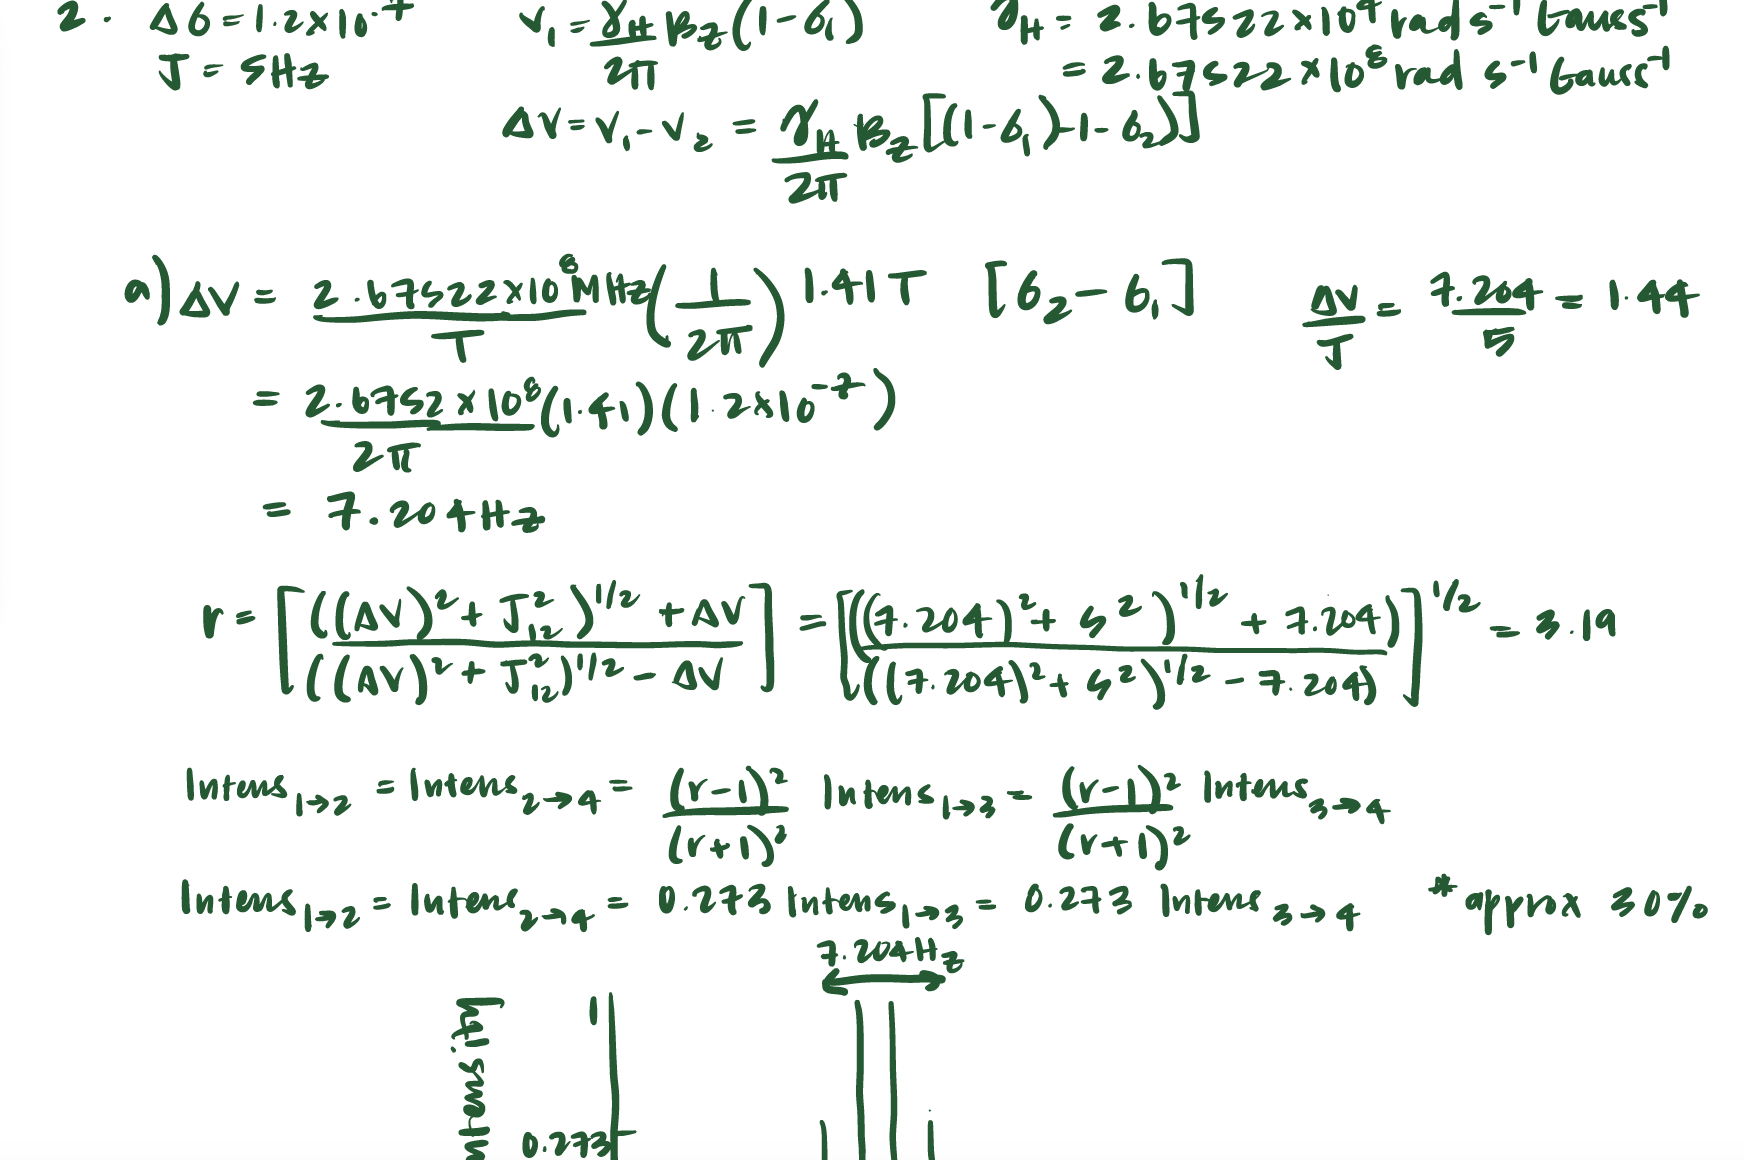
\includegraphics[width=0.8\textwidth]{2a.png}
  \caption{2a}
  \label{fig:2a}
\end{figure}
The equations to predict the relative intensities are given in 6-24 of the lecture notes. These equations predict 2 pairs of peaks with identical intensities. We get the magnetic field in Teslas by substituting the operating frequency into the Larmor equation. The $\Delta \nu$ is different for each spectrometer frequency and dictates the splitting between the center of the peaks. One would follow the same procedure for each spectrometer frequency.
\begin{figure}[H]
  \centering
  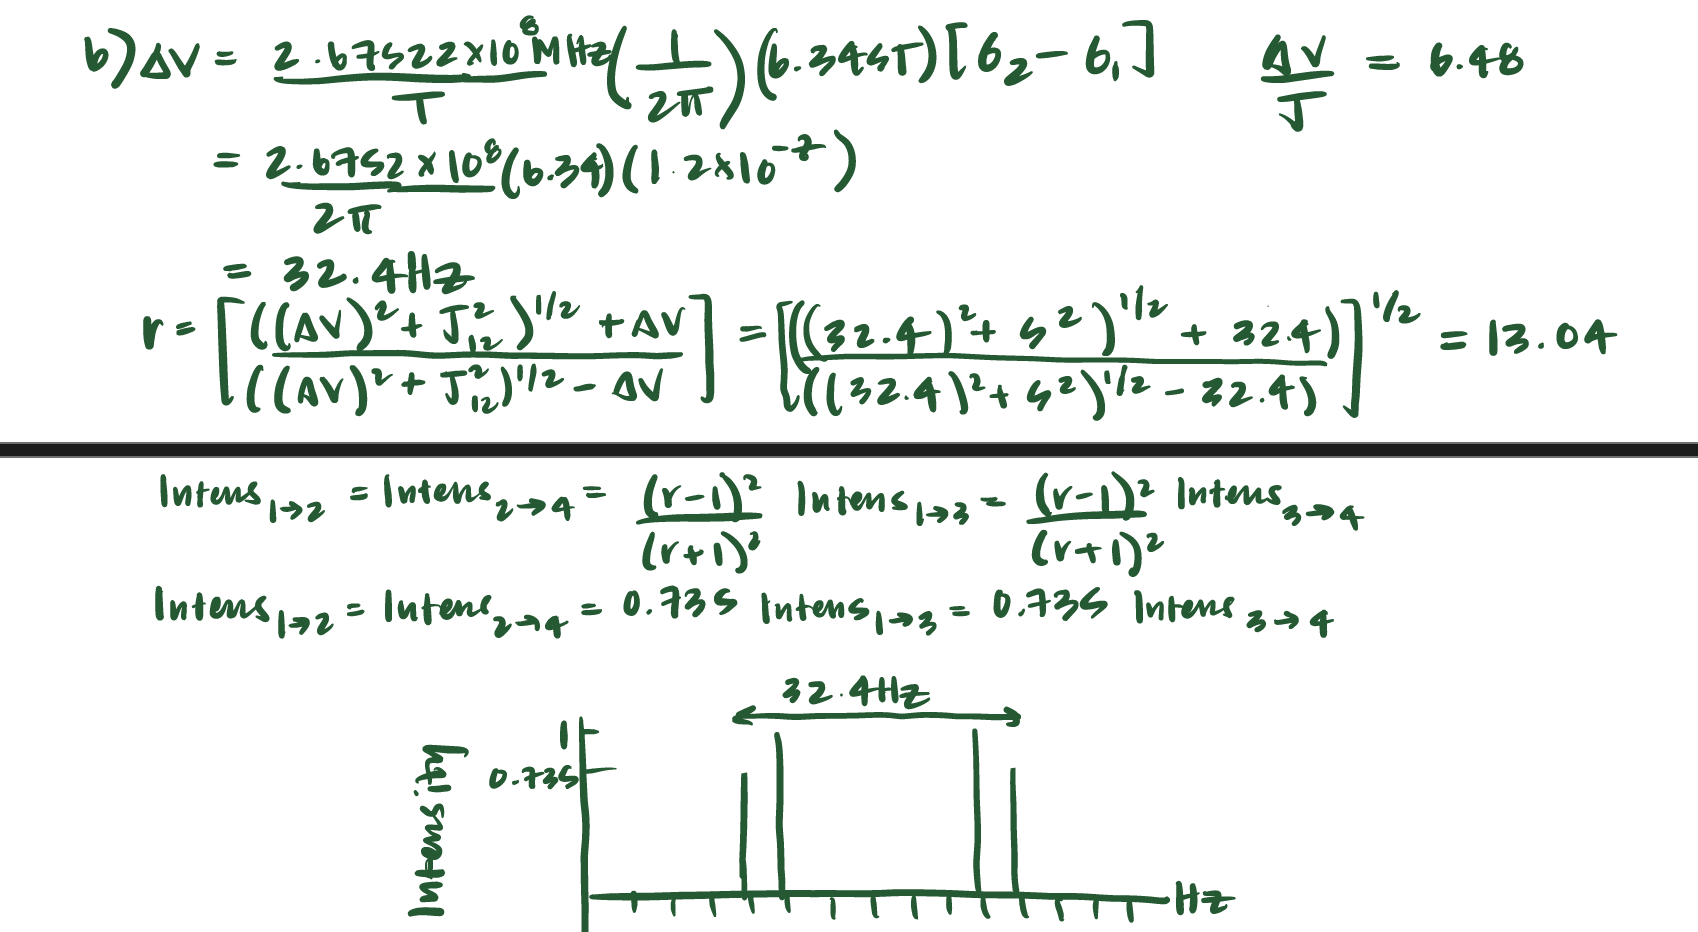
\includegraphics[width=0.8\textwidth]{2b.png}
  \caption{2b}
  \label{fig:2b}
\end{figure}
\begin{figure}[H]
  \centering
  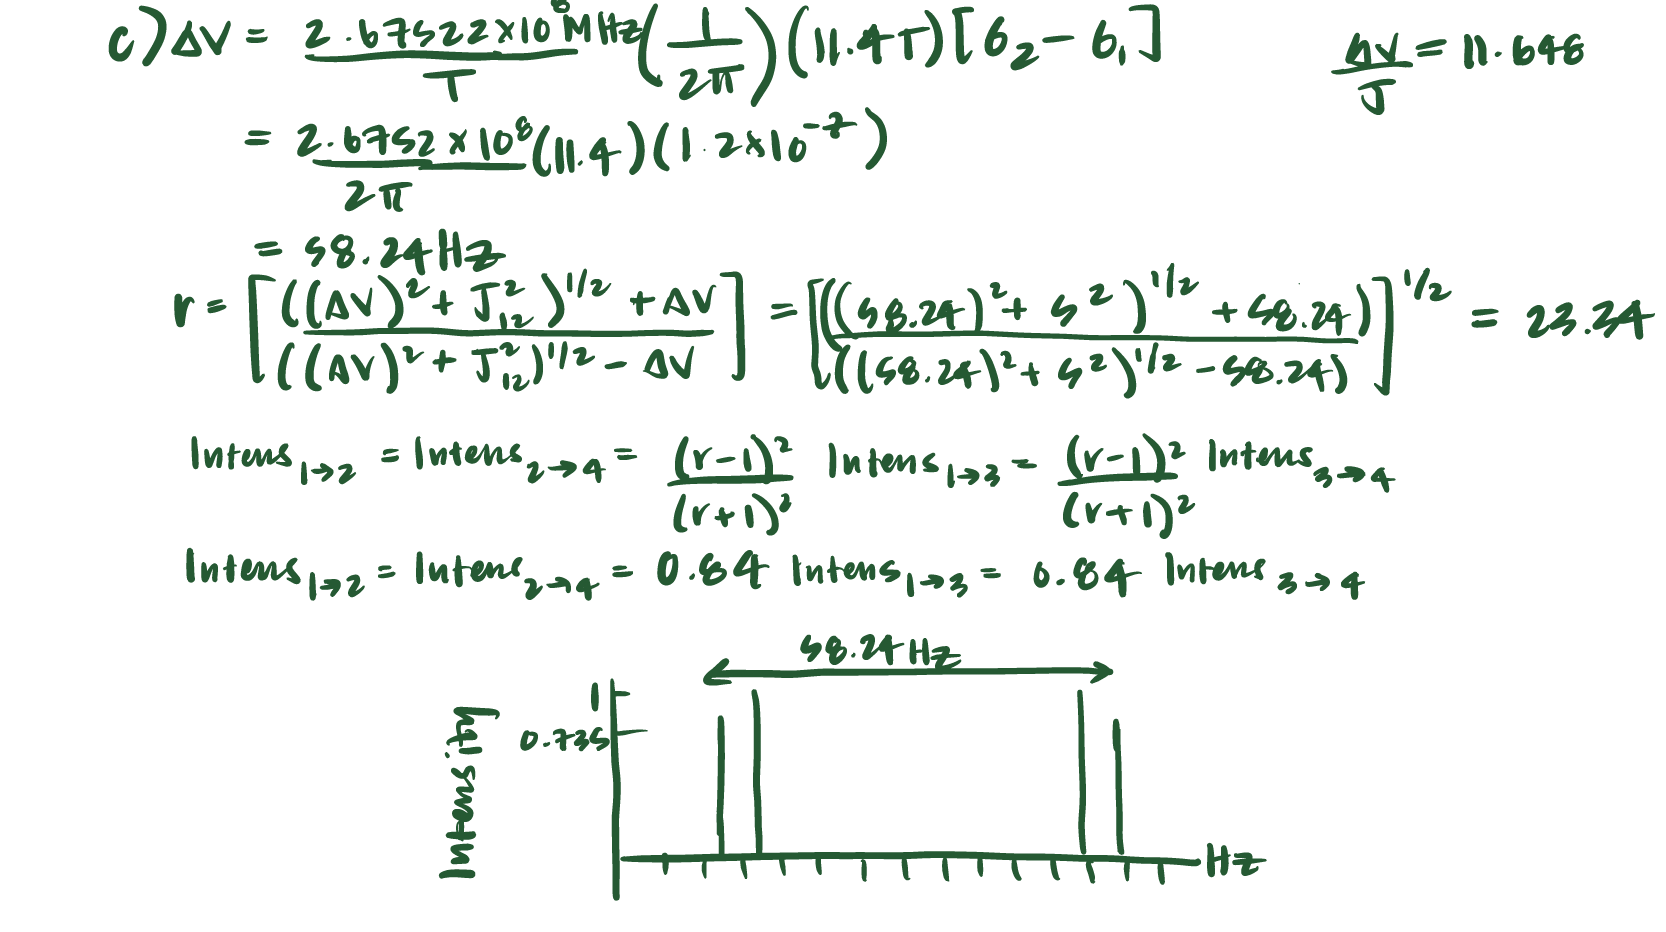
\includegraphics[width=0.8\textwidth]{2c.png}
  \caption{2c}
  \label{fig:2c}
\end{figure}
\section{}
  \item (5 points) On a certain NMR spectrometer a proton signal has a chemical shift of $5 \mathrm{ppm}$, corresponding to a frequency range of $3 \mathrm{kHz}$. What is the operating frequency of the spectrometer and what is the approximate magnetic field strength?
  The chemical shift is given by the equation:
  \begin{equation}
    \delta _{H} = \frac{\nu - \nu_{ref}}{\nu_{ref}} \times 10^6 ppm
  \end{equation}
  So we can solve for the frequency:
  \begin{equation}
    \nu{ref} = \frac{\nu - \nu_{ref}}{\delta _{H} \times 10^{-6}}
  \end{equation}
My script gives:
\begin{align}
  \nu_{ref} = 600 MHz\\
\end{align}
So the magnetic field strength is:
\begin{align}
  B_0 = \frac{2\pi \nu_{ref}}{\gamma_H}
\end{align}
My script gives:
\begin{align}
  B_0 = 14.1 T
\end{align}
% Inline Python code in the document
\begin{lstlisting}[language=Python]
import sympy as sp

# Constants
# Gyromagnetic ratio in radians s^-1 T^-1 for a proton
gamma_H = 2.6752219 * 10**8

# Given values
delta_ppm = 5  # Chemical shift in ppm
delta_hz = 3 * 10**3  # Frequency range corresponding to chemical shift in Hz

# Calculation
# Rearrange the chemical shift formula to solve for nu_0 (operating frequency)
nu_0 = sp.Symbol('nu_0')
nu = nu_0 + delta_hz
operating_frequency_equation = sp.Eq(delta_ppm, ((nu - nu_0) / nu_0) * 10**6)
operating_frequency_solution = sp.solve(operating_frequency_equation, nu_0)

# Calculate the magnetic field strength using the corrected formula
B = sp.Symbol('B')
magnetic_field_equation = sp.Eq(2 * sp.pi * operating_frequency_solution[0], gamma_H * B)
magnetic_field_strength = sp.solve(magnetic_field_equation, B)

# print with units
print("Operating frequency: {0:.2e} Hz".format(float(operating_frequency_solution[0].evalf())))
print("Magnetic field strength: {0:.2e} T".format(float(magnetic_field_strength[0].evalf())))

\end{lstlisting}
\section{}
  \item (5 points) Calculate the magnetic field strength required for ${ }^{19} \mathrm{~F}\left(\mathrm{I}=1 / 2, \gamma_{\mathrm{F}}=2.516233 \times\right.$ $10^{8}$ radians s $\left.^{-1} \mathrm{~T}^{-1}\right)$ and ${ }^{13} \mathrm{C}\left(\mathrm{I}=1 / 2, \gamma_{\mathrm{C}}=6.728286 \times 10^{7}\right.$ radians $\left.^{-1} \mathrm{~T}^{-1}\right)$ resonances in a $500 \mathrm{MHz}$ spectrometer.
  I get:
\begin{align}
  B_{0}^{F} = 12.5 T\\
  B_{0}^{C} = 46.7 T
\end{align}
% Inline Python code in the document
\begin{lstlisting}[language=Python]
import sympy as sp

# Constants
# Gyromagnetic ratios in radians s^-1 T^-1 for 19F and 13C
gamma_F = 2.516233 * 10**8  # 19F
gamma_C = 6.728286 * 10**7  # 13C
nu_0 = 500 * 10**6  # 500 MHz in Hz

# Calculation for 19F
B_F = sp.Symbol('B_F')
magnetic_field_equation_F = sp.Eq(2 * sp.pi * nu_0, gamma_F * B_F)
magnetic_field_strength_F = sp.solve(magnetic_field_equation_F, B_F)

# Calculation for 13C
B_C = sp.Symbol('B_C')
magnetic_field_equation_C = sp.Eq(2 * sp.pi * nu_0, gamma_C * B_C)
magnetic_field_strength_C = sp.solve(magnetic_field_equation_C, B_C)

# print with units
print("Magnetic field strength for 19F: {0:.2e} T".format(float(magnetic_field_strength_F[0].evalf())))
print("Magnetic field strength for 13C: {0:.2e} T".format(float(magnetic_field_strength_C[0].evalf())))

\end{lstlisting}
\section{}
  \item (5 points) Consider a two-proton spin system in which the two protons are equivalent. If the two protons are equivalent, then they are indistinguishable, and quantum mechanics requires that the wavefunction for the system is either symmetric or antisymmetric with respect to exchange of identical particles. Write down all possible orthonormal wavefunctions for this two-proton system where:

\end{enumerate}

$$
|\alpha(j)\rangle=\left|\psi_{j}(1 / 2,1 / 2)\right\rangle \quad \text { and } \quad|\beta(j)\rangle=\left|\psi_{j}(1 / 2,-1 / 2)\right\rangle
$$
We would have one singlet state:
\begin{equation}
  \ket{\psi_{singlet}} = \frac{1}{\sqrt{2}} \left( \ket{\alpha(1)\beta(2)} - \ket{\beta(1)\alpha(2)} \right)
\end{equation}
And three triplet states:
\begin{align}
  \ket{\psi_{triplet}^{1}} = \ket{\alpha(1)\alpha(2)}\\
  \ket{\psi_{triplet}^{0}} = \frac{1}{\sqrt{2}} \left( \ket{\alpha(1)\beta(2)} + \ket{\beta(1)\alpha(2)} \right)\\
  \ket{\psi_{triplet}^{-1}} = \ket{\beta(1)\beta(2)}
\end{align}
\section{}
\begin{enumerate}
  \setcounter{enumi}{5}
  \item (15 points) Assume the zero-order Hamiltonian for this spin system in a magnetic field directed along the $z$-axis of magnitude $B_{0}$ is:
\end{enumerate}

$$
\widehat{H}^{0}=-\gamma_{H} B_{0}\left(1-\sigma_{A}\right)\left(\hat{I}_{z 1}+\hat{I}_{z 2}\right)
$$

where $\sigma_{A}$ is the chemical shift parameter for the two equivalent protons. The perturbation Hamiltonian is:

$$
\widehat{H}^{\prime}=\frac{h J_{A A}}{\hbar^{2}} \hat{I}_{1} \cdot \hat{I}_{2}
$$

where $J_{A A}$ is the spin-spin coupling constant between the two protons. Using the wavefunctions from problem 5 , determined the zero-order energies and first order corrections to the energies of all four states.
\subsection{}
We start by calculating the zero-order energies. The action of the spin operators on the singlet state is:
\begin{align}
  \left(\hat{I}_{z 1} + \hat{I}_{z 2}\right) \ket{\psi_{singlet}} = \left(\hat{I}_{z 1} + \hat{I}_{z 2}\right) \frac{1}{\sqrt{2}} \left( \ket{\alpha(1)\beta(2)} - \ket{\beta(1)\alpha(2)} \right)\\
  = \frac{1}{\sqrt{2}} \left( \frac{1}{2} \ket{\alpha(1)\beta(2)} + \frac{1}{2}\ket{\beta(1)\alpha(2)} \right) + \frac{1}{\sqrt{2}} \left( -\frac{1}{2} \ket{\alpha(1)\beta(2)} - \frac{1}{2}\ket{\beta(1)\alpha(2)} \right)\\
  = 0
\end{align}
So the zero-order energy is:
\begin{equation}
  E_{singlet}^{0} = -\gamma_{H} B_{0}\left(1-\sigma_{A}\right)\left(\hat{I}_{z 1}+\hat{I}_{z 2}\right) = 0
\end{equation}
We continue with the triplet states. The action of the spin operators on the triplet state with $m_I = 1$ is:
\begin{align}
  \left(\hat{I}_{z 1} + \hat{I}_{z 2}\right) \ket{\psi_{triplet}^{1}} = \left(\hat{I}_{z 1} + \hat{I}_{z 2}\right) \ket{\alpha(1)\alpha(2)}\\
  = \frac{1}{2} \ket{\alpha(1)\alpha(2)} + \frac{1}{2} \ket{\alpha(1)\alpha(2)}\\
  = \ket{\alpha(1)\alpha(2)}
\end{align}
So the zero-order energy is:
\begin{equation}
  E_{triplet}^{1,0} = -\gamma_{H} B_{0}\left(1-\sigma_{A}\right)\left(\hat{I}_{z 1}+\hat{I}_{z 2}\right) = -\gamma_{H} B_{0}\left(1-\sigma_{A}\right)
\end{equation}
The action of the spin operators on the triplet state with $m_I = 0$ is:
\begin{align}
  \left(\hat{I}_{z 1} + \hat{I}_{z 2}\right) \ket{\psi_{triplet}^{0}} = \left(\hat{I}_{z 1} + \hat{I}_{z 2}\right) \frac{1}{\sqrt{2}} \left( \ket{\alpha(1)\beta(2)} + \ket{\beta(1)\alpha(2)} \right)\\
  = \frac{1}{\sqrt{2}} \left( \frac{1}{2} \ket{\alpha(1)\beta(2)} - \frac{1}{2}\ket{\beta(1)\alpha(2)} \right) + \frac{1}{\sqrt{2}} \left( - \frac{1}{2} \ket{\alpha(1)\beta(2)} + \frac{1}{2}\ket{\beta(1)\alpha(2)} \right)\\
  = 0
\end{align}
So the zero-order energy is:
\begin{equation}
  E_{triplet}^{0,0} = -\gamma_{H} B_{0}\left(1-\sigma_{A}\right)\left(\hat{I}_{z 1}+\hat{I}_{z 2}\right) = 0
\end{equation}
The action of the spin operators on the triplet state with $m_I = -1$ is:
\begin{align}
  \left(\hat{I}_{z 1} + \hat{I}_{z 2}\right) \ket{\psi_{triplet}^{-1}} = \left(\hat{I}_{z 1} + \hat{I}_{z 2}\right) \ket{\beta(1)\beta(2)}\\
  = -\frac{1}{2} \ket{\beta(1)\beta(2)} - \frac{1}{2} \ket{\beta(1)\beta(2)}\\
  = -\ket{\beta(1)\beta(2)}
\end{align}
So the zero-order energy is:
\begin{equation}
  E_{triplet}^{-1,0} = -\gamma_{H} B_{0}\left(1-\sigma_{A}\right)\left(\hat{I}_{z 1}+\hat{I}_{z 2}\right) = \gamma_{H} B_{0}\left(1-\sigma_{A}\right)
\end{equation}
Now we calculate the first order corrections to the energies. The spin-spin coupling operator in the perturbation Hamiltonian can be decomposed into the sum of the spin operators:
\begin{equation}
  \hat{I}_{1} \cdot \hat{I}_{2} = \hat{I}_{x 1} \hat{I}_{x 2} + \hat{I}_{y 1} \hat{I}_{y 2} + \hat{I}_{z 1} \hat{I}_{z 2}
\end{equation}
The action of the spin operators on the singlet state is:
\begin{align}
  \left(\hat{I}_{x 1} \hat{I}_{x 2} + \hat{I}_{y 1} \hat{I}_{y 2} + \hat{I}_{z 1} \hat{I}_{z 2}\right) \ket{\psi_{singlet}} = \left(\hat{I}_{x 1} \hat{I}_{x 2} + \hat{I}_{y 1} \hat{I}_{y 2} + \hat{I}_{z 1} \hat{I}_{z 2}\right) \frac{1}{\sqrt{2}} \left( \ket{\alpha(1)\beta(2)} - \ket{\beta(1)\alpha(2)} \right)\\
\end{align}
Now, we want to express the spin operators in terms of raising and lowering operators. We can do this by using the following equations:
\begin{align}
  \hat{I}_{x} = \frac{1}{2} \left( \hat{I}_{+} + \hat{I}_{-} \right)\\
  \hat{I}_{y} = \frac{1}{2i} \left( \hat{I}_{+} - \hat{I}_{-} \right)\\
\end{align}
Let us make a small table detailing the action of $\hat{I}_{+}$ and $\hat{I}_{-}$ on the states:
\begin{center}
  \begin{tabular}{ |c|c|c| } 
    \hline
    State & $\hat{I}_{+}$ & $\hat{I}_{-}$ \\
    \hline
    $\ket{\alpha}$ & 0 & $\ket{\beta}$ \\
    $\ket{\beta}$ & $\ket{\alpha}$ & 0 \\
    \hline
  \end{tabular}
\end{center}
Now, let's make another table detailing the action of $\hat{I}_{x}$ and $\hat{I}_{y}$ on the states:
\begin{center}
  \begin{tabular}{ |c|c|c|c| } 
    \hline
    State & $\hat{I}_{x}$ & $\hat{I}_{y}$ & $\hat{I}_{z}$\\
    \hline
    $\ket{\alpha}$ & $\frac{1}{2} \ket{\beta}$ & $-\frac{1}{2i} \ket{\beta}$ & $\frac{1}{2}$\\
    $\ket{\beta}$ & $\frac{1}{2} \ket{\alpha}$ & $\frac{1}{2i} \ket{\alpha}$ & $-\frac{1}{2}$\\
    \hline
  \end{tabular}
\end{center}
So the action of the spin operators on the singlet state is:
\begin{align}
  \left(\hat{I}_{x 1} \hat{I}_{x 2} + \hat{I}_{y 1} \hat{I}_{y 2} + \hat{I}_{z 1} \hat{I}_{z 2}\right) \ket{\psi_{singlet}} = \left(\hat{I}_{x 1} \hat{I}_{x 2} + \hat{I}_{y 1} \hat{I}_{y 2} + \hat{I}_{z 1} \hat{I}_{z 2}\right) \frac{1}{\sqrt{2}} \left( \ket{\alpha(1)\beta(2)} - \ket{\beta(1)\alpha(2)} \right)\\
\end{align}
With the standard basis, we get the matrix representation of the spin operators:
\begin{align}
  \hat{I}_{x} = \frac{1}{2} \begin{pmatrix}
    0 & 1\\
    1 & 0
  \end{pmatrix}\\
  \hat{I}_{y} = \frac{1}{2i} \begin{pmatrix}
    0 & -1\\
    1 & 0
  \end{pmatrix}\\
  \hat{I}_{z} = \frac{1}{2} \begin{pmatrix}
    1 & 0\\
    0 & -1
  \end{pmatrix}\\
\end{align}
The singlet state can be expressed in the standard basis as:
\begin{equation}
  \ket{\psi_{singlet}} = \frac{1}{\sqrt{2}} \left( \ket{\alpha(1)\beta(2)} - \ket{\beta(1)\alpha(2)} \right) = \left[\begin{matrix}0\\\frac{\sqrt{2}}{2}\\- \frac{\sqrt{2}}{2}\\0\end{matrix}\right]
\end{equation}
The triplet states can be expressed in the standard basis as:
\begin{align}
  \ket{\psi_{triplet}^{1}} = \ket{\alpha(1)\alpha(2)} = \left[\begin{matrix}1\\0\\0\\0\end{matrix}\right]\\
  \ket{\psi_{triplet}^{0}} = \frac{1}{\sqrt{2}} \left( \ket{\alpha(1)\beta(2)} + \ket{\beta(1)\alpha(2)} \right) = \left[\begin{matrix}0\\\frac{\sqrt{2}}{2}\\\frac{\sqrt{2}}{2}\\0\end{matrix}\right]\\
  \ket{\psi_{triplet}^{-1}} = \ket{\beta(1)\beta(2)} = \left[\begin{matrix}0\\0\\0\\1\end{matrix}\right]
\end{align}
SymPy gives the sum of these tensor products acting on the singlet state as:
\begin{equation}
  \left[\begin{matrix}0\\- 0.375 \sqrt{2}\\0.375 \sqrt{2}\\0\end{matrix}\right]
\end{equation}
And then the action on each of the triplet states:
\begin{equation}
  I_1 \cdot I_2 \ket{\psi_{triplet}^{1}} = \left[\begin{matrix}0.25\\0\\0\\0\end{matrix}\right]
\end{equation}
\begin{equation}
  I_1 \cdot I_2 \ket{\psi_{triplet}^{0}} = \left[\begin{matrix}0\\0.125 \sqrt{2}\\0.125 \sqrt{2}\\0\end{matrix}\right]
\end{equation}
\begin{equation}
  I_1 \cdot I_2 \ket{\psi_{triplet}^{-1}} = \left[\begin{matrix}0\\0\\0\\0.25\end{matrix}\right]
\end{equation}
We must note that each of the spin tensor codex contributes a factor of $\hbar$, so the first order corrections to the energies are:
\begin{align*}
  E_{\text{singlet}}^{1,1} &= \frac{h J_{AA}}{1} \bra{\psi_{\text{singlet}}}\left(\hat{I}_{x1} \hat{I}_{x2} + \hat{I}_{y1} \hat{I}_{y2} + \hat{I}_{z1} \hat{I}_{z2}\right) \ket{\psi_{\text{singlet}}} = -0.75 \frac{h J_{AA}}{1}\\
  E_{\text{triplet}}^{1,1} &= \frac{h J_{AA}}{1} \bra{\psi_{\text{triplet}}^{1}}\left(\hat{I}_{x1} \hat{I}_{x2} + \hat{I}_{y1} \hat{I}_{y2} + \hat{I}_{z1} \hat{I}_{z2}\right) \ket{\psi_{\text{triplet}}^{1}} = 0.25 \frac{h J_{AA}}{1}\\
  E_{\text{triplet}}^{1,-1} &= \frac{h J_{AA}}{1} \left(\hat{I}_{x1} \hat{I}_{x2} + \hat{I}_{y1} \hat{I}_{y2} + \hat{I}_{z1} \hat{I}_{z2}\right) \ket{\psi_{\text{triplet}}^{-1}} = 0.25 \frac{h J_{AA}}{1}\\
  E_{\text{triplet}}^{1,0} &= \frac{h J_{AA}}{1} \left(\hat{I}_{x1} \hat{I}_{x2} + \hat{I}_{y1} \hat{I}_{y2} + \hat{I}_{z1} \hat{I}_{z2}\right) \ket{\psi_{\text{triplet}}^{0}} = 0.25 \frac{h J_{AA}}{1}
\end{align*}
% Inline Python code in the document
\begin{lstlisting}[language=Python]
from sympy import Matrix, sqrt, I, latex
from sympy.physics.quantum import TensorProduct, Dagger

# Define basis states
alpha = Matrix([[1], [0]])
beta = Matrix([[0], [1]])

# Define singlet state
psi_singlet = 1/sqrt(2) * (TensorProduct(alpha, beta) - TensorProduct(beta, alpha))
psi_triplet_1 = TensorProduct(alpha, alpha)
psi_triplet_0 = 1/sqrt(2) * (TensorProduct(alpha, beta) + TensorProduct(beta, alpha))
psi_triplet_m1 = TensorProduct(beta, beta)


# Define spin operators in matrix form
Ix = 1/2 * Matrix([[0, 1], [1, 0]])
Iy = 1/(2*I) * Matrix([[0, 1], [-1, 0]])
Iz = 1/2 * Matrix([[1, 0], [0, -1]])

# loop over all states and find the digonal matrix elements of the spin operators
for psi in [psi_singlet, psi_triplet_1, psi_triplet_0, psi_triplet_m1]:
    print("Psi =")
    print(latex(psi))
    for I in [Ix, Iy, Iz]:
        print("I =")
        print(latex(I))
    # get the combined sum of the spin operators like \left(\hat{I}_{x1} \hat{I}_{x2} + \hat{I}_{y1} \hat{I}_{y2} + \hat{I}_{z1} \hat{I}_{z2}\right) 
    # we want to use the TensorProduct function to get the diagonal matrix elements of the combined sum
    big_I = TensorProduct(Ix, Ix) + TensorProduct(Iy, Iy) + TensorProduct(Iz, Iz)
    # calculate the diagonal matrix elements of the combined sum with both the bra and ket being the same state
    singlet_result = Dagger(psi) * big_I * psi
    # print the result
    print("singlet_result =")
    print(latex(singlet_result))
\end{lstlisting}


\begin{enumerate}
  \setcounter{enumi}{6}
  \item (5 points) Using the wavefunctions from the problem 5 , identify all of the allowed NMR transitions among them. How many lines do you expect to see in the proton NMR spectrum of this system?
\end{enumerate}
Since the total swim has to be conserved only transitions among the triplet state are allowed. Additionally, transitions must have $\Delta m_I \pm 1$. So there are two allowed transitions:
\begin{align}
  \ket{\psi_{triplet}^{1}} \rightarrow \ket{\psi_{triplet}^{0}}\\
  \ket{\psi_{triplet}^{0}} \rightarrow \ket{\psi_{triplet}^{-1}}
\end{align}
You would expect to see 2 lined, corresponding to these transitions.
\end{document}